\chapter{模型如何学习：损失函数与优化}
在前两章中，我们已经把一个预测问题整理成了样本、特征和目标，也学会了用表格保存数据。接下来遇到的问题是：把这些数据交给一个模型之后，究竟发生了什么？程序为什么能够从一条位置不合适的直线，得到一条更贴近数据的直线？软件中的 \texttt{fit} 看起来只有一行，但要正确使用模型，需要知道这一行在解决什么问题。

本章所说的\textbf{优化}，是按照已经规定的数值目标寻找更合适参数的过程；目标变小表示这个训练准则得到改善，不自动表示模型在新数据上更可靠。

本章围绕一条直线回答这些问题。我们先说明哪些量可以调整，再用损失函数规定调整的方向，最后通过梯度下降观察参数怎样一步步变化。采用简单模型，是为了让预测、误差和更新之间的关系都可以直接看见。今后处理多个特征、概率输出或多层神经网络时，这条思路仍然有用；具体的模型表达、目标函数和求解方法则会改变。

本章有两类教学材料。一类是人为规定的单参数损失函数，用来观察学习率；另一类是程序人工生成的直线数据，用来观察完整训练过程。它们都不是物理测量或天文观测。真实科学问题还涉及测量不确定性、样本选择、对象之间的关联以及适用范围，不能由一幅漂亮的拟合图替代。本章先集中解决``模型怎样学到参数''，第4章再系统讨论``学到的模型表现怎样''。

\section*{学习目标}

学完本章，应能完成以下工作：

1. 指出一个简单模型的输入、输出和可学习参数，区分模型表达、训练目标与优化方法。

2. 从预测误差构造损失，解释经验损失与正则化项各自的作用。

3. 根据梯度完成一两步参数更新，解释学习率、特征尺度和停止条件对训练过程的影响。

4. 区分全批量、随机和小批量更新，区分模型参数与超参数，并提交可复现的参数记录与损失曲线。

\section{模型表达与可学习参数}

\subsection{从一个输入到一个预测}

设我们希望用一个数值输入 \(x\) 预测一个连续目标 \(y\)。例如，在某个有限的工作范围内，可以尝试用输入信号预测传感器的输出。开始建模时，需要先提出一个可计算的关系。本章选择最简单的直线：

\[\widehat{y} = f(x;a,b) = ax + b.\]

这里，\(x\) 是输入特征，\(\widehat{y}\) 是模型给出的预测值，\(a\) 是斜率，\(b\) 是截距。帽子符号提醒我们，\(\widehat{y}\) 是计算结果，不是数据中已经给出的目标 \(y\)。斜率决定输入改变一个单位时预测改变多少，截距决定 \(x = 0\) 时的预测。若输入和目标有物理单位，斜率和截距也随之具有相应单位；本章人工数据中的两个变量均为无量纲量。

表达式 \(ax + b\) 定义了一族可能的直线，还没有确定具体使用哪一条。取不同的 \(a\) 和 \(b\)，就会得到不同的预测关系。模型训练的任务，是依据训练数据和预先规定的准则，在这些可能的直线中寻找合适的一条。这里能够通过训练调整的量 \(a\)、\(b\)，称为\textbf{模型参数}。为了方便书写，可把它们合在一个二维参数向量中，记为 \(\mathbf{\theta} = (a,b)^{\mathsf{T}}\)；上标 \(\mathsf{T}\) 表示转置，使其写成列向量。

改变参数和改变模型形式是两种不同操作。调整 \(a\) 或 \(b\)，所得曲线仍然是一条直线；如果改用二次多项式，就引入了新的表达能力和新的参数。训练不能让一个坚持使用直线的模型自动变成任意弯曲的函数。因此，当数据关系明显弯曲而模型始终只能画直线时，仅仅增加训练次数并不能消除表达能力的限制。

\subsection{数据在训练中的位置}

用 \(\left( x_{i},y_{i} \right)\) 表示第 \(i\) 条训练记录，其中 \(i = 1,2,\ldots,n\)，\(n\) 是训练记录数。给定一组参数后，模型对这条记录的预测是 \({\widehat{y}}_{i} = ax_{i} + b\)。训练期间，数据中的 \(x_{i}\) 和 \(y_{i}\) 保持不变，变化的是参数和由它们计算出来的预测。把目标列也放进输入，或者为了让曲线更好看而修改目标值，都不属于这里讨论的参数学习。

在第1章的任务分类中，这属于\textbf{有监督学习中的回归任务}：训练记录同时给出输入和数值目标。无监督学习没有同样的监督目标列，但仍可能学习某种结构，并通过自己的目标函数进行拟合。因此，``有损失函数''不等于``必然有监督''，``使用梯度下降''也不能用来判断一个任务属于监督还是无监督。本章只选择有监督回归作为解释训练机制的起点。

图3-1给出了同一批人工训练记录和几条候选直线。灰黑色散点始终相同，改变的是直线的位置。观察这些直线时，可以先凭直觉判断哪一条更贴近数据，再思考怎样把这个判断交给程序。人眼能看二维散点，程序却需要一个明确的数值准则；下一节的损失函数就是连接这两者的工具。

\begin{figure}[htbp]\centering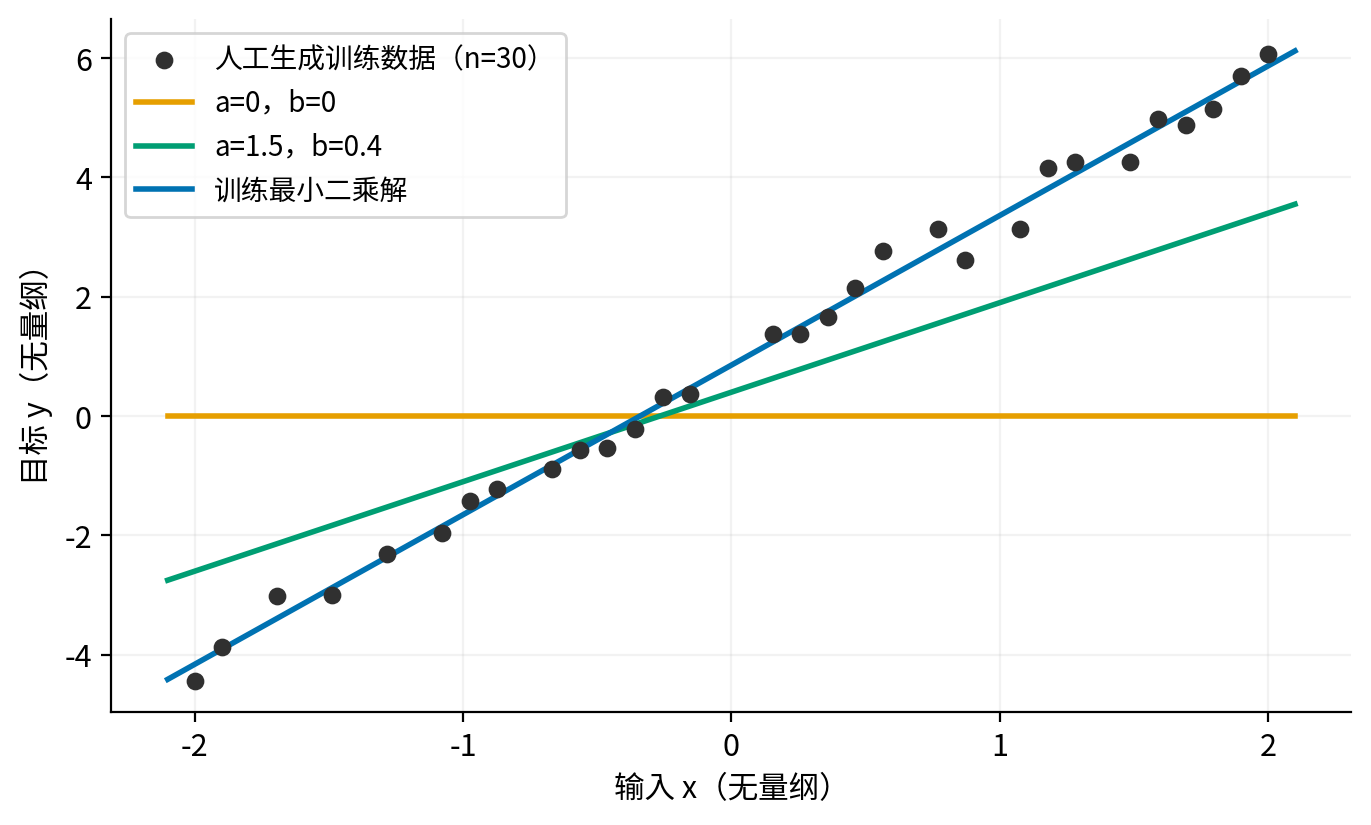
\includegraphics[width=0.92\linewidth]{figures/ch03_figure_1.png}\caption{人工生成数据中固定的30条训练记录，输入与目标均无量纲。三条直线属于相同模型形式。图中的训练最小二乘解仅作为后续求解的参照，未使用其余10条保留记录。}\end{figure}

\subsection{模型、目标和优化方法各回答什么}

在讨论一个学习算法时，最好把三个问题分别说清楚。模型表达回答``怎样从输入得到预测''；训练目标回答``怎样衡量当前参数是否合适''；优化方法回答``怎样寻找使目标较小的参数''。表3-1把本章的选择放在一起，后续章节会逐步替换其中的内容。

表3-1 本章训练问题的三个组成部分

\begin{longtable}[]{@{}
  >{\raggedright\arraybackslash}p{(\columnwidth - 4\tabcolsep) * \real{0.1441}}
  >{\raggedright\arraybackslash}p{(\columnwidth - 4\tabcolsep) * \real{0.3314}}
  >{\raggedright\arraybackslash}p{(\columnwidth - 4\tabcolsep) * \real{0.5245}}@{}}
\toprule\noalign{}
\begin{minipage}[b]{\linewidth}\raggedright
\textbf{组成部分}
\end{minipage} & \begin{minipage}[b]{\linewidth}\raggedright
\textbf{本章的具体选择}
\end{minipage} & \begin{minipage}[b]{\linewidth}\raggedright
\textbf{它规定的事情}
\end{minipage} \\
\midrule\noalign{}
\endhead
\bottomrule\noalign{}
\endlastfoot
模型表达 & \(\widehat{y} = ax + b\) & 给定输入与参数后怎样预测 \\
训练目标 & 训练数据上的半均方误差 & 怎样比较不同参数的拟合程度 \\
优化方法 & 梯度下降 & 怎样依据当前参数计算下一步参数 \\
\end{longtable}

同一个模型可以有不同的求解方法；同一种优化方法也能用于不同模型。梯度下降属于优化方法，不能与逻辑回归、决策树等预测模型放在同一层级上理解。sklearn 的官方说明也特别区分了随机梯度下降与由它训练的模型。{[}1{]} 到第5章，我们会比较线性回归的求解路径；到第6章，模型输出将与类别概率联系起来，但``模型---目标---求解''的区分仍然成立。

\subsection{模型形式、目标函数与求解方法是三个选择}
对同一批直线数据，可以保持模型$\hat y=ax+b$不变，分别最小化平方误差和绝对误差；也可以保持平方误差目标不变，分别采用直接最小二乘求解和梯度下降。前一种比较改变了“什么参数算好”，后一种比较改变了“怎样找到这些参数”。若两者同时改变，结果差异就不能仅归因于优化器。

这个区分解释了为什么一个软件接口只有一行，背后却有多层选择。\texttt{fit}是统一的操作名称，输入包括数据和配置，输出是已拟合状态；它不承诺内部一定执行固定次数的梯度更新。近邻方法保存并组织训练记录，决策树比较候选划分，普通最小二乘可以用矩阵分解。后面每章都需要分别回答模型、目标与学习过程这三个问题。

\section{从预测误差到损失函数}

\subsection{为什么不能直接平均正负误差}

给定一个预测，最直接的误差是预测与目标之差。本章采用统一约定：

\[e_{i} = {\widehat{y}}_{i} - y_{i}.\]

\(e_{i}\) 称为第 \(i\) 条记录的残差。它为正，表示预测偏高；为负，表示预测偏低。也有书籍采用相反的残差符号，只要在损失和求导中保持一致即可。这里明确符号，是为了让后面的更新方向可以逐项核对。

考虑表3-2中的三个点。它们是专为手算构造的无噪声例子，与后面的40条CSV记录相互独立。真实关系在此被直接设定为 \(y = 2x + 1\)，当前模型却取 \(a = 1,b = 1\)。

表3-2 用于手算的人工三点例子

\begin{longtable}[]{@{}
  >{\raggedright\arraybackslash}p{(\columnwidth - 8\tabcolsep) * \real{0.1657}}
  >{\raggedright\arraybackslash}p{(\columnwidth - 8\tabcolsep) * \real{0.1657}}
  >{\raggedright\arraybackslash}p{(\columnwidth - 8\tabcolsep) * \real{0.2377}}
  >{\raggedright\arraybackslash}p{(\columnwidth - 8\tabcolsep) * \real{0.1945}}
  >{\raggedright\arraybackslash}p{(\columnwidth - 8\tabcolsep) * \real{0.2363}}@{}}
\toprule\noalign{}
\begin{minipage}[b]{\linewidth}\raggedright
\textbf{输入} \(x_{i}\)
\end{minipage} & \begin{minipage}[b]{\linewidth}\raggedright
\textbf{目标} \(y_{i}\)
\end{minipage} & \begin{minipage}[b]{\linewidth}\raggedright
\textbf{当前预测} \({\widehat{y}}_{i}\)
\end{minipage} & \begin{minipage}[b]{\linewidth}\raggedright
\textbf{残差} \(e_{i}\)
\end{minipage} & \begin{minipage}[b]{\linewidth}\raggedright
\textbf{残差平方} \(e_{i}^{2}\)
\end{minipage} \\
\midrule\noalign{}
\endhead
\bottomrule\noalign{}
\endlastfoot
\(- 1\) & \(- 1\) & \(0\) & \(1\) & \(1\) \\
\(0\) & \(1\) & \(1\) & \(0\) & \(0\) \\
\(1\) & \(3\) & \(2\) & \(- 1\) & \(1\) \\
\end{longtable}

三条残差的平均值是0，但其中两条预测并不正确。这说明平均带符号误差可以反映整体偏高或偏低，却不能独自衡量预测偏离的大小。正负误差可能相互抵消。若把每个残差先平方再平均，偏高和偏低都会产生非负的代价，抵消就不会发生。

本章把单条记录的损失定义为：

\[\ell_{i} = \frac{1}{2}\left( {\widehat{y}}_{i} - y_{i} \right)^{2} = \frac{1}{2}e_{i}^{2}.\]

这里的 \(\ell_{i}\) 是该记录的\textbf{平方损失}，系数 \(1/2\) 是为了使后面的导数更简洁。对 \(n\) 条训练记录取平均，得到：

\[J(a,b) = \frac{1}{n}\sum_{i = 1}^{n}\ell_{i} = \frac{1}{2n}\sum_{i = 1}^{n}\left( ax_{i} + b - y_{i} \right)^{2}.\]

\(J\) 是当前参数在整批训练记录上的\textbf{半均方误差}。表3-2中，\(J = (1 + 0 + 1)/(2 \times 3) = 1/3\)。通常所说的均方误差，即 MSE，没有前面的 \(1/2\)，因此本例 MSE 为 \(2/3\)。本章所有标为``训练损失''的直线实验都采用半均方误差，不能把图中的数值直接当作未经换算的 MSE。

\subsection{损失函数表达了怎样的偏好}

平方并不只是消除了符号。它还使较大的残差受到较重的惩罚：残差的绝对值加倍，平方项变为原来的四倍。因此，少数偏离较远的记录可能明显影响最终直线。面对实验数据中的异常读数时，这种性质既可能帮助模型认真处理大偏差，也可能使错误记录牵动拟合结果。选择损失函数，就是规定模型怎样看待不同类型的预测错误。

平方损失不是唯一选择。绝对损失使用残差绝对值，其他损失可以在小残差和大残差区域采用不同惩罚。分类任务的输出和目标含义不同，也需要适合该任务的目标函数。第6章讨论逻辑回归时，我们会从概率预测引出相应损失，而不会直接把类别编号当作普通连续测量值来套用本章例子。这里先把一种损失理解透彻，比提前记住许多名称更有用。

损失的量纲和数值大小也要结合目标理解。如果 \(y\) 表示某个带单位的测量量，平方损失就带有该单位的平方。把目标由一种单位换成另一种单位，即使预测关系在物理上没有改变，损失数字也会变化。因此，不同任务的损失大小通常不能直接横向比较。在科学数据中，各条记录还可能有不同的测量不确定性，是否应赋予不同权重，需要结合误差模型另行判断。本章的等权平均只对应所有训练记录采用相同权重的教学设定。

\subsection{训练损失与评价指标的联系}

训练损失直接参与参数寻找；评价指标用于回答模型表现的问题。二者可以使用相同的数学形式，但使用的数据和承担的任务仍需区分。例如，MSE既可以与回归训练目标有关，也可以在未参与训练的数据上计算，作为评价结果。反过来，有些便于解释的评价指标并不适合直接用于梯度更新。

本章反复绘制的曲线使用的都是训练记录。它们告诉我们优化过程有没有改善当前训练目标，不能独自说明模型能否预测新对象。一个算法把训练损失降得很低，可能是学到了稳定关系，也可能过度适应了当前样本；这需要额外证据区分。先把``当前数据上拟合得怎样''与``新数据上表现怎样''分开，后续的验证、测试和泛化概念就更容易理解。

\section{经验损失 正则化与训练目标}

\subsection{从有限样本出发的目标}

我们希望模型在未来遇到的样本上也有较小误差，但未来所有可能的样本并没有同时摆在面前。训练时能够直接计算的，是已有训练样本上的平均损失。因此，上一节的 \(J\) 也称为\textbf{经验损失}。``经验''指它来自有限数据，并不表示它只是凭经验随意规定的数值。损失的形式由建模者选择，损失的具体数值则由数据和当前参数共同决定。

一旦训练数据和模型形式固定，每一组参数都有一个对应的经验损失。训练就是在参数空间中寻找较小的目标值。对于一条直线，参数空间有两个方向：一个方向改变斜率，另一个方向改变截距。不能因为数据散点画在 \(x\)、\(y\) 平面里，就把寻找参数想象成移动某条数据记录；优化所移动的是参数空间中的位置。

为什么不总是追求把训练损失降到零？首先，模型形式可能无法穿过所有点。其次，数据中的随机噪声不一定具有可预测性。更复杂的模型虽然可能把每条训练记录都贴得很近，却未必更适合后续样本。要理解这种取舍，除了选择模型形式，还需要认识另一种控制方式：正则化。

\subsection{在拟合误差之外增加约束偏好}

在本章的直线例子中，可在经验损失上增加一个与斜率大小有关的项：

\[J_{\lambda}(a,b) = J(a,b) + \frac{\lambda}{2}a^{2},\quad\quad\lambda \geq 0.\]

\(J_{\lambda}\) 表示加入正则化后的训练目标，\(\lambda\) 是控制惩罚强弱的非负数。这里使用平方型惩罚，是 L2 正则化的一个简单例子；为了突出斜率的作用，本例不惩罚截距。不同模型和软件对截距的处理可能不同，不能把这一约定当作全部方法的统一规则。本章的 \(\lambda\) 专指上述``半均方误差加 \(\lambda a^{2}/2\)''的定义，不直接等同于所有 sklearn 估计器中的同名或类似选项；第5章会结合具体目标解释 Ridge 的 \texttt{alpha}。

当 \(\lambda = 0\) 时，目标只包含经验损失；当 \(\lambda > 0\) 时，算法除了希望拟合误差小，还要付出斜率过大的代价。参数调整需要平衡这两部分，而不是先把直线拟合好，再随意把斜率改小。正则化改变的是训练要解决的问题，所以通常也会改变最终参数。

利用本章30条人工训练记录，直接求解上述二次目标，可得到表3-3。这里的计算用于认识训练目标，不涉及保留数据上的表现。表中的数值按实际运行结果取六位小数。

表3-3 不同正则化强度对应的训练解，原始输入坐标，截距不惩罚

\begin{longtable}[]{@{}
  >{\raggedright\arraybackslash}p{(\columnwidth - 8\tabcolsep) * \real{0.1081}}
  >{\raggedright\arraybackslash}p{(\columnwidth - 8\tabcolsep) * \real{0.1801}}
  >{\raggedright\arraybackslash}p{(\columnwidth - 8\tabcolsep) * \real{0.1801}}
  >{\raggedright\arraybackslash}p{(\columnwidth - 8\tabcolsep) * \real{0.2305}}
  >{\raggedright\arraybackslash}p{(\columnwidth - 8\tabcolsep) * \real{0.3012}}@{}}
\toprule\noalign{}
\begin{minipage}[b]{\linewidth}\raggedright
\(\lambda\)
\end{minipage} & \begin{minipage}[b]{\linewidth}\raggedright
\textbf{斜率} \(a\)
\end{minipage} & \begin{minipage}[b]{\linewidth}\raggedright
\textbf{截距} \(b\)
\end{minipage} & \begin{minipage}[b]{\linewidth}\raggedright
\textbf{经验损失} \(J\)
\end{minipage} & \begin{minipage}[b]{\linewidth}\raggedright
\textbf{正则化项} \(\lambda a^{2}/2\)
\end{minipage} \\
\midrule\noalign{}
\endhead
\bottomrule\noalign{}
\endlastfoot
0 & 2.506900 & 0.853364 & 0.026641 & 0.000000 \\
0.1 & 2.342148 & 0.873641 & 0.045935 & 0.274283 \\
1.0 & 1.471686 & 0.980775 & 0.788396 & 1.082930 \\
\end{longtable}

随着惩罚增强，斜率向0收缩，经验损失却变大了。这并不说明优化失败：算法优化的是包含惩罚项的整个目标。不同 \(\lambda\) 对应不同目标函数，也不能把它们各自的目标最小值直接排在一起，选数值最小者作为最佳正则化强度。应当怎样选择强度、怎样检验它是否改善新样本上的表现，是第4章和第5章要进一步解决的问题。

正则化是一种建模偏好，不能替代科学知识。对于本例，它鼓励较小的斜率，却没有自动判断哪个斜率符合某条物理定律。斜率的数字还依赖输入单位；改用不同尺度的输入，同一预测关系可能对应很不一样的参数大小。因此，特征处理、正则化形式和强度需要一起理解。第3.8节的尺度实验先考察没有正则化时的优化过程，以免同时改变太多因素。

\subsection{训练目标清楚之后，仍需选择求解方法}

写出目标函数，并不意味着只能通过梯度下降求解。对于结构简单的最小二乘问题，可以利用专门的数值线性代数方法；对于其他问题，可能使用不同的迭代优化或结构搜索。本章训练直线时亲手写出梯度下降，是为了把参数更新过程展开来看。

在 sklearn 中，\texttt{fit} 是统一接口名称，表示估计器根据数据完成拟合，它不保证内部使用某一种优化方法。本章传入普通稠密数据、保持默认非负约束设置时，\texttt{LinearRegression} 使用最小二乘数值求解，并不默认执行后面所写的梯度下降循环。{[}2{]} 所以，仅凭代码出现了 \texttt{model.fit(X,\ y)}，无法判断它怎样学习；需要结合模型与求解器的说明。

这一点也关系到后续神经网络学习。梯度下降利用梯度更新参数；反向传播则是对神经网络这类复合计算高效计算梯度的方法。两者承担不同工作。第12章会在本章的更新规则之上解释梯度怎样逐层得到，这里先集中理解``给定梯度后怎样改变参数''。

\section{导数 梯度与参数变化}

\subsection{导数告诉我们局部变化方向}

先只考虑一个可调整参数 \(w\)，把目标写成 \(J(w)\)。导数 \(J'(w)\) 描述：在当前位置附近，参数发生很小变化时，目标大致怎样变化。若 \(J'(w) > 0\)，在足够小的范围内增大 \(w\) 会使目标增大，因此可以尝试减小 \(w\)；若 \(J'(w) < 0\)，则可以尝试增大 \(w\)。这里反复强调``附近''和``足够小''，因为导数是局部信息，并不保证任意大的一步都有效。

用一个小改变量 \(\Delta w\) 表示参数的移动，可以把这个关系简写为：

\[J(w + \Delta w) \approx J(w) + J'(w)\Delta w.\]

式中，\(\Delta w\) 越小，局部线性近似通常越有用。要让右侧的变化项为负，可以让 \(\Delta w\) 与导数符号相反。这就是沿负导数方向更新的直觉来源。但近似式没有告诉我们具体该走多远；步长还需由下一节的学习率控制。

本章用以下人为规定的函数作示意：

\[J(w) = \frac{1}{2}(w - 3)^{2},\quad\quad J'(w) = w - 3.\]

这里的 \(w\) 只是示意参数，\(J\) 也不是由CSV数据计算得到的损失。我们特意把最小点设在 \(w = 3\)，以便直接核对更新方向。若 \(w = 0\)，导数为 \(- 3\)，应尝试增大参数；若 \(w = 4\)，导数为1，应尝试减小参数。越靠近3，导数的绝对值越小。在这个简单例子中，梯度也自然提供了``接近谷底时减小移动幅度''的信息。

\subsection{多个参数需要一个方向向量}

直线模型有两个参数，只知道改变斜率的影响还不够。我们分别考察保持 \(b\) 不变而改变 \(a\)，以及保持 \(a\) 不变而改变 \(b\) 时，目标怎样变化。这两个变化率称为偏导数。把它们组成向量，就得到\textbf{梯度}：

\[\nabla J(a,b) = \begin{pmatrix}
\frac{\partial J}{\partial a} \\
\frac{\partial J}{\partial b}
\end{pmatrix}.\]

\(\nabla\) 是表示梯度的符号。它的两个分量分别对应斜率方向和截距方向，顺序必须与参数向量 \((a,b)^{\mathsf{T}}\) 一致。在当前参数坐标采用通常的欧氏距离时，梯度指向局部增大目标最快的方向，负梯度则给出相反方向。改变参数的数值尺度，会改变这种几何关系，这也是标准化可能影响优化的重要原因。

对本章的半均方误差，只需保留下面两条实用公式：

\[\frac{\partial J}{\partial a} = \frac{1}{n}\sum_{i = 1}^{n}e_{i}x_{i},\quad\quad\frac{\partial J}{\partial b} = \frac{1}{n}\sum_{i = 1}^{n}e_{i}.\]

其中，\(e_{i} = ax_{i} + b - y_{i}\) 是当前参数产生的残差。截距每增加一点，会同样改变所有预测，因此它的梯度是平均残差；斜率的改变对不同输入的影响不同，所以它的梯度还包含 \(x_{i}\)。理解这两个分量的来源，比只记住公式更能帮助我们检查代码。

回到表3-2。当前残差为1、0、\(- 1\)，输入为\(- 1\)、0、1。因此，斜率方向的梯度为\(( - 1 + 0 - 1)/3 = - 2/3\)，截距方向的梯度为0。模型没有整体向上或向下平移的需要，但斜率偏小，需要增大。这也解释了为什么``平均残差为0''并不表示已经找到最优直线：它只能使这里的截距梯度为0，斜率梯度仍然不为0。

\subsection{怎样理解梯度接近零}

若所有梯度分量都接近零，沿很小的参数变化已经难以获得明显的一阶下降。对于本章这种输入并不全相同的直线最小二乘问题，损失面呈碗形，存在唯一最小点，因此小梯度是接近最优解的重要信号。对于复杂模型，目标面可能出现不同结构，梯度为零也可能对应其他驻点，不能不加条件地解释为找到了全局最优模型。

在实际计算中，还要留意梯度与数据处理的联系。若输入中有极大的数值，斜率梯度中的 \(e_{i}x_{i}\) 也可能很大；若数据里有异常目标，残差本身可能主导更新。梯度不是脱离数据的抽象箭头，它把当前模型、目标定义和样本数值联系起来。观察梯度异常时，应当同时检查这些来源，而不是只反复增加迭代次数。

\subsection{用数值差分检查解析梯度}
复杂模型的梯度公式可能写错。一个不依赖同一推导的检查办法，是直接轻微改变参数，观察目标变化。对第$j$个参数，中心差分近似为
\[
\frac{\partial J}{\partial\theta_j}\approx
\frac{J(\boldsymbol\theta+\varepsilon\mathbf e_j)-J(\boldsymbol\theta-\varepsilon\mathbf e_j)}{2\varepsilon},
\]
其中$\mathbf e_j$只在第$j$个位置为1。这个方法需要两次目标计算，而不是调用已写好的梯度函数，因此能够发现许多符号、系数和求和方向错误。$\varepsilon$太大时截断误差明显，太小时浮点减法可能丢失有效数字；教学中可用$10^{-4},10^{-5},10^{-6}$检查结果是否稳定。

新增检查采用三点$x=(1,2,3)$、$y=(3,5,8)$，初始斜率1、截距0，目标为\emph{MSE}而非本章基础实验的半MSE。解析梯度为$(-46/3,-20/3)$，中心差分与之吻合。这里专门改用MSE，是为了再次核对目标定义：乘在目标前的常数会改变梯度，却不改变无正则情况下的最小点。代码与公式必须使用同一个约定。

数值差分检查通过不代表整个模型正确。它主要说明当前位置附近的目标函数和梯度实现相容，仍需检查数据、目标定义及评价过程。对于分段不可导点，应避开拐点或明确采用的导数约定，第12章将在ReLU网络上再次使用这一检查。

\section{梯度下降 学习率与停止条件}

\subsection{从方向得到一次更新}

有了梯度，还需要决定每次沿该方向移动多少。令 \(\eta > 0\) 表示\textbf{学习率}，\(t\) 表示已经完成的更新次数，梯度下降写成：

\[\mathbf{\theta}^{(t + 1)} = \mathbf{\theta}^{(t)} - \eta\nabla J\left( \mathbf{\theta}^{(t)} \right).\]

\(\mathbf{\theta}^{(t)}\) 是第 \(t\) 步参数，右侧梯度也必须在这一组旧参数上计算。对直线来说，应先算出两个梯度分量，再同时更新 \(a\) 和 \(b\)。若先改变 \(a\)，再用新 \(a\) 计算 \(b\) 的梯度，就已经改变了这里定义的更新规则。

表3-2的例子可立即用于一次检查。取学习率 \(\eta = 0.3\)，从 \(a = 1,b = 1\) 出发，由于梯度为 \(( - 2/3,0)^{\mathsf{T}}\)，更新后得到 \(a = 1.2,b = 1\)。新的残差为0.8、0、\(- 0.8\)，半均方误差从 \(1/3\) 降为 \(0.64/3 \approx 0.213333\)。这个短计算把方向、步长、预测和损失连成了一条完整链条。

再看单参数示意函数。从 \(w^{(0)} = 0\) 出发，取 \(\eta = 0.5\)，有：

\[\begin{matrix}
w^{(1)} & = 0 - 0.5 \times (0 - 3) = 1.5, \\
w^{(2)} & = 1.5 - 0.5 \times (1.5 - 3) = 2.25.
\end{matrix}\]

两步之后，损失依次由4.5降到1.125，再降到0.28125。参数逐渐接近3，梯度的绝对值也随之减小。这里没有使用``知道答案以后直接把参数设成3''的做法，程序每一步只依据当前位置的导数行动。

\subsection{学习率过小、合适和过大}

图3-2比较了四个学习率，初始位置和示意目标完全相同。学习率0.1的参数一直从左侧接近最小点，但12步后仍只有约2.152711。学习率0.5接近得更快，12步后约为2.999268。学习率1.5每一步都会跨过最小点，参数在两侧交替，不过偏离幅度越来越小。学习率2.1也左右交替，却越走越远，12步后的损失约44.323797，高于起点的4.5。

\begin{figure}[htbp]\centering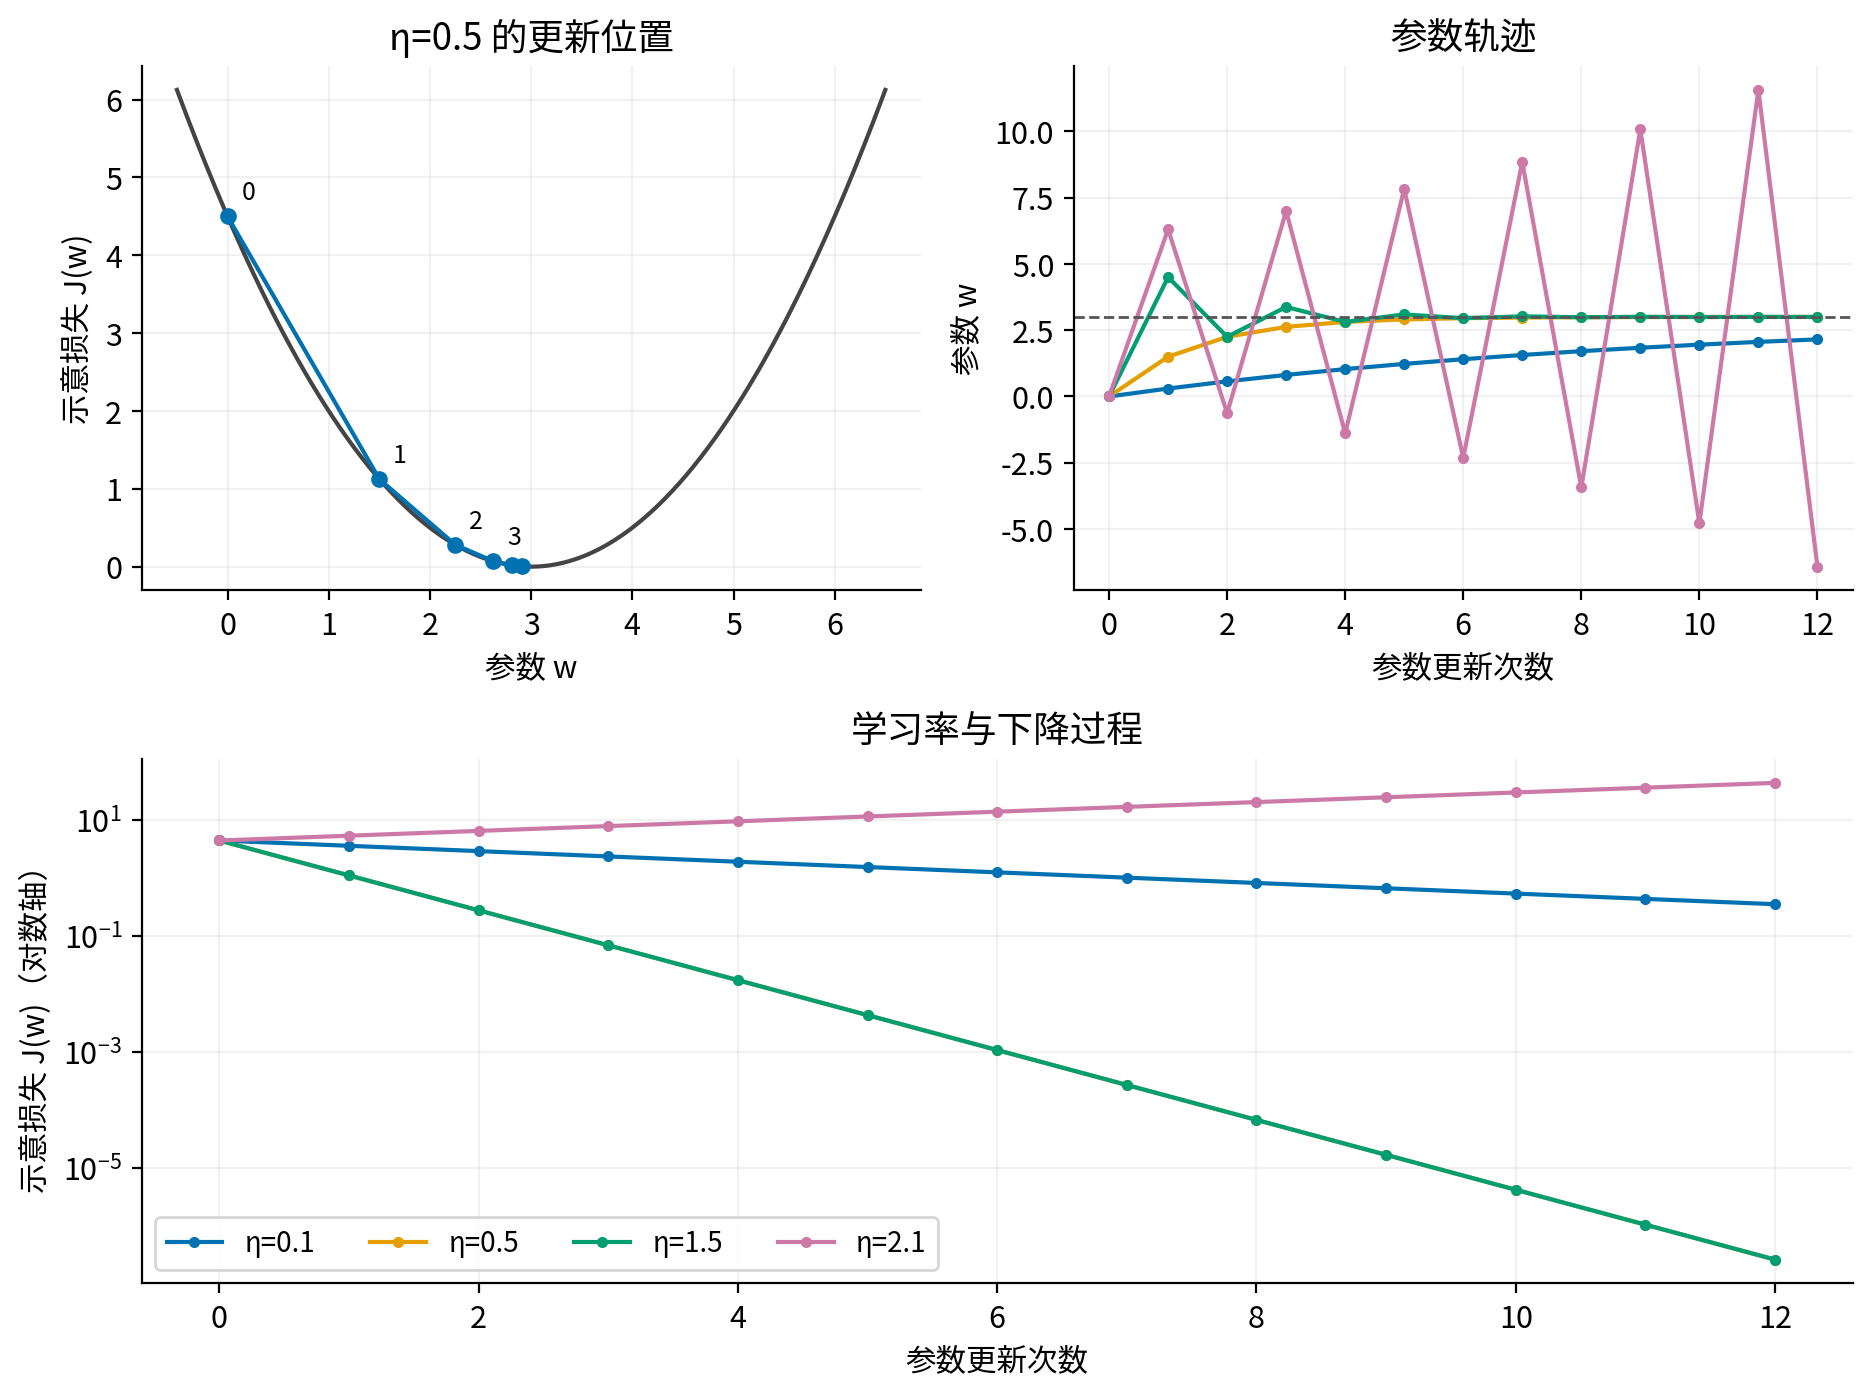
\includegraphics[width=0.92\linewidth]{figures/ch03_figure_2.png}\caption{人为设定的示意损失 \(J(w) = (w - 3)^{2}/2\)，不使用任何观测或训练记录。上左图标出学习率0.5的前几步位置，其横轴为参数 \(w\)；上右图显示参数轨迹，下图显示损失轨迹，两者横轴均为参数更新次数。下图采用对数纵轴；学习率0.5与1.5的损失曲线完全重合。}\end{figure}

这个例子说明，出现振荡不一定意味着发散。应当看振荡幅度是缩小、保持还是放大，也要观察损失怎样变化。对于本例，把更新式整理一下，可以得到：

\[w^{(t + 1)} - 3 = (1 - \eta)\left( w^{(t)} - 3 \right).\]

因此，学习率0.5和1.5虽然轨迹不同，偏离最小点的绝对值每一步都减半，损失曲线恰好重合。学习率2.0会使参数在0和6之间来回，损失保持4.5。这个边界取决于当前示意函数的形状，不能据此说``所有任务的学习率小于2就安全''。换一个目标、换一种特征尺度，适合的学习率都可能改变。

同样需要注意目标前面的常数。如果把半均方误差改成MSE，最小点不变，梯度却整体扩大一倍。在没有同步调整学习率时，更新轨迹就会改变。这是比较不同教材、软件或代码时经常遇到的细节：数值上相同的学习率，只有在目标定义和更新规则也一致时才具有相同意义。

\subsection{何时停止，以及停止意味着什么}

最直观的停止方式是规定最大更新次数。它容易实现，可以限制计算量，但``用完了次数''只说明程序执行结束，不说明一定接近最小点。另一种方式是观察相邻若干步的目标变化是否很小，或梯度范数是否小于设定阈值。梯度范数是把多个梯度分量合起来衡量其大小的量。设置这些阈值时，要考虑目标和参数的尺度，不能把某个小数机械地复制到所有问题。

损失变平也需要解释。如果学习率极小，参数几乎没有移动，曲线可能很平，却仍离最优值很远；若计算达到浮点精度所能分辨的范围，继续迭代也可能没有可见改善。因此，判断训练状态时，最好同时查看目标、参数变化和必要的参照值，而不是只看图是否平滑。

本章直线基础实验固定执行120次更新，方便不同学生复现同一轨迹。这个次数是教学中的停止设置，程序并没有利用保留数据决定何时停止。尺度实验另设损失超过 \(10^{12}\) 时的保护停止，以防明显发散继续造成数值问题；这种停止代表需要检查学习率或输入尺度，绝不表示成功收敛。第4章会进一步说明利用验证数据观察泛化表现的做法，它与这里仅检查训练优化状态的停止判断承担不同任务。

\subsection{选读：一个能精确分析的收敛条件}
对二次目标$J(\boldsymbol\theta)=\frac12(\boldsymbol\theta-\boldsymbol\theta^*)^{\mathsf T}H(\boldsymbol\theta-\boldsymbol\theta^*)+c$，假定$H$为对称正定矩阵。$H$称为Hessian矩阵，记录目标对参数的二阶变化，在本例中为常数。设误差$\mathbf e_t=\boldsymbol\theta_t-\boldsymbol\theta^*$，梯度更新成为
\[
\mathbf e_{t+1}=(I-\eta H)\mathbf e_t.
\]
沿$H$的一个特征向量方向，误差每步乘以$1-\eta\lambda_j$。要让各方向的误差都缩小，需要所有$|1-\eta\lambda_j|<1$，因此可用的恒定学习率满足
\[
0<\eta<\frac{2}{\lambda_{\max}(H)}.
\]
这一推导只用了对称矩阵特征分解，不要求证明一般非线性优化定理。它说明最陡方向限制了步长，而较平缓方向可能仍然走得很慢。不同方向曲率相差很大时，一个共同步长难以兼顾，这为特征缩放提供了定量解释。

在上节新增的三点MSE例子中，设计矩阵每行为$(x_i,1)$，$H=2D^{\mathsf T}D/3$，其最大特征值约11.09294，因此这一个二次问题的稳定上界约为0.180295。不能把这个数复制到其他数据，也不能把二次正定模型的结论无条件推广到所有神经网络。神经网络的局部曲率随参数变化，非凸问题还存在不同驻点。

这一分析也澄清“负梯度是最快下降方向”的条件：它是当前点的一阶局部描述，并以欧氏长度约束步长方向。走有限的一大步仍可能越过低处。方向选择、步长选择与全局是否收敛是相关但不同的问题。

\section{批量 随机与小批量更新}

\subsection{每次梯度可以用多少条记录}

前面的直线梯度由全部 \(n\) 条训练记录的平均贡献计算得到。每更新一次，都遍历全部训练记录，这叫\textbf{全批量梯度下降}，也常简称批量梯度下降。它使我们看到当前训练目标的完整梯度；在本章的二次目标上配合足够小的学习率，可以得到平稳的下降过程。当样本很多时，每次更新前都处理全部记录的计算开销也会增大。

另一种办法是每次只使用一条记录的损失梯度进行更新，称为\textbf{随机梯度下降}，英文缩写为 SGD。实践中可以随机抽取记录，也可以在每轮开始时打乱顺序，再依次使用每条记录。本章采用后一种方式。它让参数在读完全部记录之前就多次变化，但单条记录的方向未必与完整训练梯度相同。

在两者之间，可以把记录分成若干较小的批次，每次用一批记录的平均梯度更新，这就是\textbf{小批量梯度下降}。设当前批次的索引集合为 \(B\)，批次大小为 \(m = |B|\)，则直线模型的两个梯度分量改写为：

\[g_{a} = \frac{1}{m}\sum_{i \in B}^{}e_{i}x_{i},\quad\quad g_{b} = \frac{1}{m}\sum_{i \in B}^{}e_{i}.\]

这里的残差都由当前参数计算。批次大小等于 \(n\) 时退回全批量，等于1时成为单样本更新。若最后一批不足预设大小，应按实际包含的记录数取平均。不能一边改变批次大小，一边仍除以固定的训练样本总数，否则也改变了梯度的数值尺度。

\subsection{一次更新与一轮遍历不同}

\textbf{一次迭代}在本章中专指一次参数更新；\textbf{一轮}，即 epoch，表示训练记录完整参与一次遍历。以30条训练记录为例，全批量每轮只更新1次，批量大小为6时每轮更新5次，单样本更新每轮则更新30次。因此，规定``训练80轮''与规定``更新80次''完全不同。

表3-4给出本章批量实验的计数。三种方式采用相同的初始参数、相同的常数学习率0.1和同一份训练标准化数据，均遍历80轮。这样，每种方式都有2400次样本参与更新，但更新次数不同。图中记录完整训练损失所增加的计算不计入样本访问量，因此这些数目也不能直接当作实际耗时。

表3-4 三种批量方式的计算安排

\begin{longtable}[]{@{}
  >{\raggedright\arraybackslash}p{(\columnwidth - 8\tabcolsep) * \real{0.1441}}
  >{\raggedright\arraybackslash}p{(\columnwidth - 8\tabcolsep) * \real{0.2089}}
  >{\raggedright\arraybackslash}p{(\columnwidth - 8\tabcolsep) * \real{0.1945}}
  >{\raggedright\arraybackslash}p{(\columnwidth - 8\tabcolsep) * \real{0.2017}}
  >{\raggedright\arraybackslash}p{(\columnwidth - 8\tabcolsep) * \real{0.2508}}@{}}
\toprule\noalign{}
\begin{minipage}[b]{\linewidth}\raggedright
\textbf{方式}
\end{minipage} & \begin{minipage}[b]{\linewidth}\raggedright
\textbf{每次更新使用记录数}
\end{minipage} & \begin{minipage}[b]{\linewidth}\raggedright
\textbf{每轮更新次数}
\end{minipage} & \begin{minipage}[b]{\linewidth}\raggedright
\textbf{80轮更新次数}
\end{minipage} & \begin{minipage}[b]{\linewidth}\raggedright
\textbf{参与更新的样本总次数}
\end{minipage} \\
\midrule\noalign{}
\endhead
\bottomrule\noalign{}
\endlastfoot
全批量 & 30 & 1 & 80 & 2400 \\
小批量 & 6 & 5 & 400 & 2400 \\
随机 & 1 & 30 & 2400 & 2400 \\
\end{longtable}

这一比较控制了数据遍历量，却没有使三种方法的全部条件都等价。例如，它们更新参数的频率不同，适合的学习率设置也未必相同。设计对照实验时，应该先说明要控制什么，再解释结果。本章用这些条件呈现不同更新方式的特点，不把一个小数据实验当作一般性的速度排名。

\subsection{为什么损失曲线会有波动}

在第3.8节的图3-5中，我们在每次更新后都用全部30条训练记录计算半均方误差。这样，三条曲线的纵坐标具有同一含义。小批量或单样本梯度可能使当前批次的拟合改善，却让其他记录的拟合稍差，所以完整训练损失不保证每一步都下降。观察到某一步上升，不能立即认定程序有误；应结合上升幅度、长期趋势和更新方式判断。

当参数已经接近最小点时，这种区别更加明显。全批量梯度接近零，并不意味着每一条记录的梯度都接近零。含噪声的数据通常不可能被同一条直线全部穿过，单条记录仍会把参数拉向不同方向。使用不变的学习率时，随机更新因而可能在最小点附近持续波动。减小后期学习率或使用其他策略可以改变这种现象，但也会引入新的设置，本章教师Notebook保留一个递减学习率的选做例子。

本次固定打乱种子为42时，全批量、小批量和随机方式的末步训练半均方误差分别约为0.02664172、0.02664471和0.02734320。更换打乱种子为0至4，随机方式的末步结果在约0.02689578至0.02984611之间变化。在这组固定设置下，随机和小批量方式的末步参数会受到样本顺序影响；全批量方式在本程序中不打乱顺序，其结果不随该种子变化。不能据此宣布某种方法在所有任务中更好。

实践中，``SGD''有时也被宽泛地用于包含小批量的随机优化方法。阅读资料时要查看实际批量大小，而不是只看名称。sklearn 的 \texttt{SGDRegressor} 则是一个采用随机梯度学习线性模型的具体估计器，不能把其默认设置与本章手写循环直接视为相同。{[}1{]} 本章先明确每次用多少条记录、怎样取平均和怎样计步，后续再学习具体工具的参数就不容易混淆。

\subsection{随机梯度为什么可以估计完整梯度}
若每条训练记录等概率被抽取，单样本梯度的平均满足
\[
\mathbb E_i[\nabla\ell_i(\boldsymbol\theta)]
=\frac1n\sum_{i=1}^n\nabla\ell_i(\boldsymbol\theta)=\nabla J(\boldsymbol\theta)
\]
（这里$J$指数据平均损失）。于是随机梯度虽然一次可能朝向不同方向，在上述抽样条件和固定参数处，其期望等于完整梯度。对独立均匀抽取的小批量，批梯度平均具有同样性质。\textbf{被用来估计梯度的是梯度向量，不是标量损失值本身。}

实践中每轮打乱后无放回遍历，与每步独立有放回抽样并不完全相同。由于参数不断改变，也不能简单把一轮全部更新等同于在同一个参数点计算完整梯度。这个差别无需在入门时展开证明，但可以通过改变样本顺序观察不同轨迹。

重复同一个随机种子得到相同轨迹，是复现检查；改变随机种子考察末步参数与验证表现的波动，是稳定性检查。二者都需要做，但回答的问题不同。不能只汇报恰好收敛最快或误差最低的种子。

\section{模型参数与超参数}

\subsection{哪些量由拟合得到，哪些量由我们设置}

斜率 \(a\) 和截距 \(b\) 根据训练数据更新，是本章的模型参数。学习率、批量大小、最大更新次数和正则化强度则需要在一次训练开始前给出，或者按照预先规定的规则变化，通常称为\textbf{超参数}。表3-5列出两类量的区别。它们都影响结果，但进入学习流程的位置不同。

表3-5 本章常见数量的角色

\begin{longtable}[]{@{}
  >{\raggedright\arraybackslash}p{(\columnwidth - 4\tabcolsep) * \real{0.2738}}
  >{\raggedright\arraybackslash}p{(\columnwidth - 4\tabcolsep) * \real{0.2449}}
  >{\raggedright\arraybackslash}p{(\columnwidth - 4\tabcolsep) * \real{0.4813}}@{}}
\toprule\noalign{}
\begin{minipage}[b]{\linewidth}\raggedright
\textbf{数量}
\end{minipage} & \begin{minipage}[b]{\linewidth}\raggedright
\textbf{角色}
\end{minipage} & \begin{minipage}[b]{\linewidth}\raggedright
\textbf{在本章中的获得方式}
\end{minipage} \\
\midrule\noalign{}
\endhead
\bottomrule\noalign{}
\endlastfoot
斜率 \(a\)、截距 \(b\) & 模型参数 & 由训练记录与求解方法确定 \\
学习率 \(\eta\) & 优化超参数 & 在训练前设置或规定变化日程 \\
批量大小 & 优化超参数 & 规定每次更新使用多少条记录 \\
最大更新次数 & 训练停止设置 & 给定计算预算上限 \\
正则化强度 \(\lambda\) & 训练目标的超参数 & 控制误差与参数惩罚的权衡 \\
标准化均值与尺度 & 预处理的已学习状态 & 只由训练输入计算 \\
随机种子 & 复现设置 & 控制数据生成或打乱过程 \\
\end{longtable}

把某个量称为超参数，不意味着它不能通过数据辅助选择，而是说它不属于当前这一次拟合直接优化的那组模型参数。例如，可以比较几个学习率或正则化强度，但怎样比较、用哪些数据比较，需要一个独立于单次训练的选择流程。若反复查看本应保留的数据来选择设置，就破坏了其后续作为独立评价依据的作用。第4章会给出规范的模型选择流程，本章只观察训练机制，不利用保留记录调参。

有些设置改变学习的路径，有些设置改变学习的问题。学习率主要影响怎样寻找当前目标的较小值；正则化强度改变目标本身；选择直线或二次模型则改变可用的表达形式。如果把这些设置同时修改，即使最后损失不同，也很难说清原因。因此，初学阶段的对照实验应尽量一次改变一个明确因素，并记录其他条件。

\subsection{数据预处理也有从训练数据获得的状态}

标准化通常要先计算训练输入的均值和尺度，再把输入转成新的坐标。均值和尺度并不是模型的斜率、截距，但它们同样是从数据中得到的已学习状态。预测后续样本时，应沿用训练阶段得到的变换，不能每遇到一批新数据就自行重新定义坐标。

以 \texttt{StandardScaler} 为例，先在训练数据上 \texttt{fit}，再对需要处理的数据 \texttt{transform}。在尚未划分数据时就对全部记录拟合标准化器，会让保留部分参与流程的建立。sklearn 的实践文档明确要求先划分、再从训练部分学习预处理变换。{[}3{]} 本章已把40条人工记录固定划分为30条训练记录与10条保留记录，尺度实验的均值和尺度只来自训练记录。训练记录由固定随机索引确定，并不连续占据CSV的前30行，因此实际操作应以 \texttt{split\ ==\ \textquotesingle{}train\textquotesingle{}} 选行。保留记录虽然随数据包保存，仍不参与本章拟合、标准化或结果评价。

\subsection{阅读 sklearn 的参数名称}

软件接口中的 \texttt{parameter} 一词比本节的``模型参数''更宽。在 sklearn 中，构造估计器时传入的设置，以及 \texttt{get\_params()} 返回的内容，通常对应我们需要配置的选项；拟合后学到的系数则常保存为带结尾下划线的属性。例如，\texttt{LinearRegression} 拟合后的 \texttt{coef\_} 和 \texttt{intercept\_} 分别保存系数和截距。{[}2{]} 因此，不能因为接口把某个选项叫 parameter，就把它直接等同于通过损失最小化学到的权重。

具体计数方式也要查清。某个工具的 \texttt{max\_iter} 可能按数据遍历轮数计，另一个求解器则按内部迭代计，不能只看名称便假设它们完全一致。本章手写程序直接使用 \texttt{steps} 表示更新次数、\texttt{epochs} 表示遍历轮数，目的就是把这个差别显式表达出来。后续使用成熟估计器时，也应能从文档找到对应含义。

固定随机种子能够帮助复现给定环境中的一次运行，但它不能证明结果稳定。数据生成、数据划分和训练打乱也最好分别记录，避免只写一个含义不清的``随机种子''。当研究问题涉及随机波动时，还需要比较多个种子或多个合理划分。复现一次结果与证明结论稳健，是两项相互联系但并不相同的工作。

\section{一次可视化的模型训练实验}

\subsection{明确数据与本次实验的问题}

现在把前面的概念串成一次可重复的训练实验。我们要观察三个变化：参数从何处出发、拟合线如何移动、训练损失如何改变。基础实验保持模型形式和损失函数固定，再分别改变特征尺度及批量方式。运行之前先写下预测，运行之后用参数和曲线解释现象。

配套的 \texttt{line\_data.csv} 包含40条人工记录。输入在 \(\lbrack - 2,2\rbrack\) 上等间距取值，目标按下面的公式生成：

\[y_{i} = 2.5x_{i} + 0.8 + \varepsilon_{i},\quad\quad\varepsilon_{i} \sim \mathcal{N}\left( 0,{0.3}^{2} \right).\]

\(\varepsilon_{i}\) 是独立抽取的随机扰动，\(\mathcal{N}\left( 0,{0.3}^{2} \right)\) 表示均值为0、标准差为0.3的正态分布。这个噪声模型是为了构造可解释的小实验而设定的，不能当作所有物理或天文数据的通用误差模型。噪声生成种子为2026，划分种子为20261114，两者相互独立。固定划分中有30条训练记录，其余10条在本章保留不用。

文件包含 \texttt{sample\_id}、\texttt{x}、\texttt{y}、\texttt{split} 四列。身份字段与划分字段帮助追踪记录，但不作为模型输入。完整字段说明随数据提供。若把 \texttt{sample\_id} 编成数字送进模型，训练问题就与当前设计不同了；若把 \texttt{split} 当作特征，划分标记也会被错误地带入预测关系。

学生Notebook已经提供路径设置与依赖导入。读取并选择训练记录的关键代码为：

\begin{verbatim}
table = pd.read_csv(ROOT / "data" / "line_data.csv")
train = table.loc[table["split"].eq("train")].copy()
x = train["x"].to_numpy()
y = train["y"].to_numpy()
\end{verbatim}

Pandas表格用于识别列和筛选记录，NumPy数组用于计算。本例中 \texttt{x} 和 \texttt{y} 都是一维数组，各有30个元素。在调用 sklearn 估计器时，输入特征仍需保留二维结构，因此使用 \texttt{train{[}{[}"x"{]}{]}}；只有一个特征并不意味着样本维度可以省略。

\subsection{记录参数与训练损失}

初始参数设为 \(a = b = 0\)，学习率设为0.2，每一步使用全部30条训练记录。梯度函数直接对应第3.4节公式：

\begin{verbatim}
def gradient(x, y, theta):
    error = theta[0] * x + theta[1] - y
    return np.array([
        np.mean(error * x),
        np.mean(error)
    ])
\end{verbatim}

其中 \texttt{theta{[}0{]}} 保存斜率，\texttt{theta{[}1{]}} 保存截距。更新时只需写 \texttt{theta\ =\ theta\ -\ lr\ *\ gradient(x,\ y,\ theta)}。完整Notebook在更新前后保存参数和训练损失，且把初始化记录为第0步；这样，图中的第1步始终表示已经完成一次更新，不会与第一次打印记录混淆。

表3-6摘取了实际运行中的几个时刻。第1步之后，斜率和截距已朝正确方向移动；第5步时主要趋势已经出现；第20步后，剩余变化在图上很难分辨。第120步的半均方误差约为0.02664148，并没有降到零。

表3-6 全批量梯度下降的参数记录，30条人工训练记录，学习率0.2

\begin{longtable}[]{@{}
  >{\raggedright\arraybackslash}p{(\columnwidth - 6\tabcolsep) * \real{0.1729}}
  >{\raggedright\arraybackslash}p{(\columnwidth - 6\tabcolsep) * \real{0.2305}}
  >{\raggedright\arraybackslash}p{(\columnwidth - 6\tabcolsep) * \real{0.2305}}
  >{\raggedright\arraybackslash}p{(\columnwidth - 6\tabcolsep) * \real{0.3660}}@{}}
\toprule\noalign{}
\begin{minipage}[b]{\linewidth}\raggedright
\textbf{更新次数}
\end{minipage} & \begin{minipage}[b]{\linewidth}\raggedright
\textbf{斜率} \(a\)
\end{minipage} & \begin{minipage}[b]{\linewidth}\raggedright
\textbf{截距} \(b\)
\end{minipage} & \begin{minipage}[b]{\linewidth}\raggedright
\textbf{训练半均方误差}
\end{minipage} \\
\midrule\noalign{}
\endhead
\bottomrule\noalign{}
\endlastfoot
0 & 0.000000 & 0.000000 & 5.168790 \\
1 & 0.741376 & 0.232381 & 2.593654 \\
5 & 2.074561 & 0.673205 & 0.186735 \\
20 & 2.505119 & 0.850248 & 0.026649 \\
120 & 2.506900 & 0.853364 & 0.026641 \\
\end{longtable}

\begin{figure}[htbp]\centering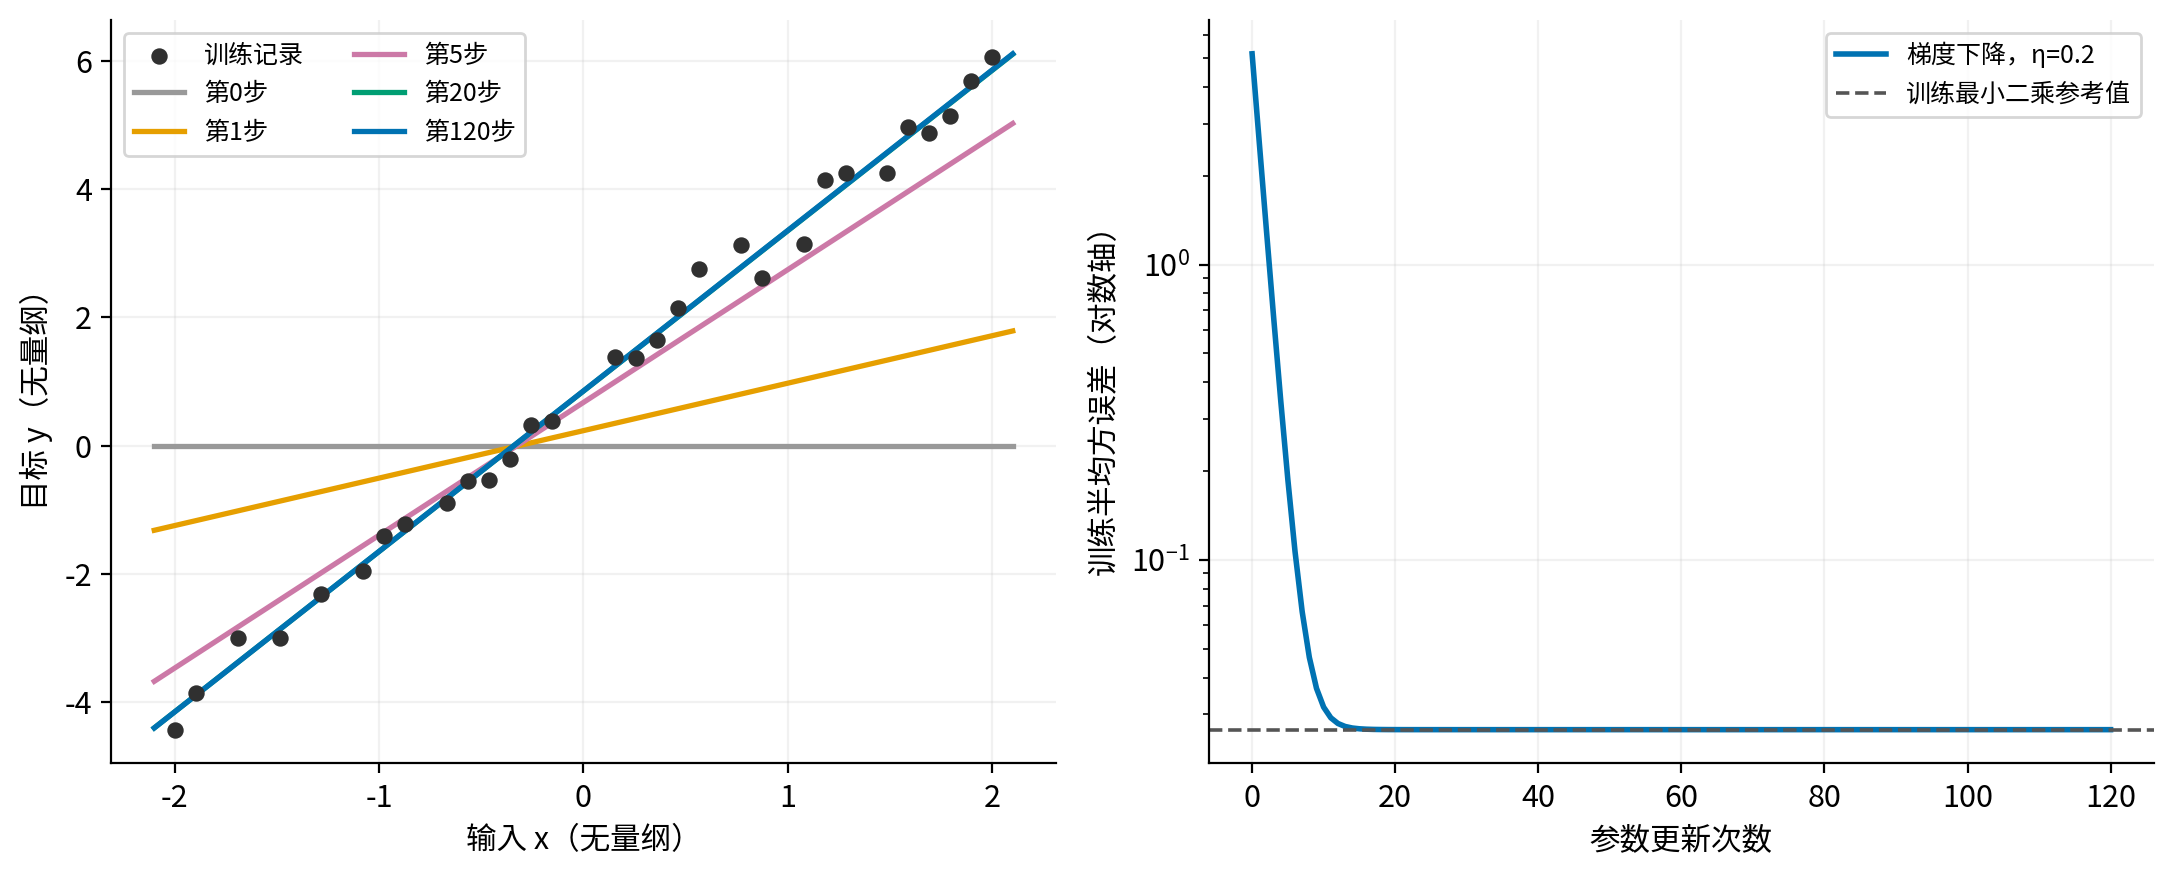
\includegraphics[width=0.92\linewidth]{figures/ch03_figure_3.png}\caption{仅使用固定的30条人工训练记录。左图展示初始状态和若干更新时刻的直线，输入与目标均无量纲；右图展示训练半均方误差及同一训练目标的最小二乘参考值，纵轴为对数轴。参数从 \((0,0)\) 出发，学习率为0.2，共更新120次。}\end{figure}

怎样判断当前低损失是不是因为代码恰好写错了？在这个结构简单的问题上，可以用独立的求解路径作参照。使用 \texttt{LinearRegression} 拟合同样的输入与目标，得到的斜率约为2.506900，截距约为0.853364。手写梯度下降在120步后与其参数的最大绝对差约为 \(1.13 \times 10^{- 12}\)。两种方法共同求解同一个无正则化目标，结果相符支持了本例实现的正确性；这一参照方法并不要求所有机器学习问题都有直接解。

还要区分拟合参数与生成参数。生成式中的斜率和截距是2.5、0.8，而训练得到的是另一组相近数值。这是有限训练样本包含随机噪声的结果。模型寻找的是当前30条记录上的最小损失直线，没有被告知应当直接返回生成式。训练损失不为零也很自然，因为一条直线不能同时穿过全部含噪声的点。已有结果支持``优化过程接近了当前目标的最小值''，尚未检验``在新的观测条件下足够准确''。

\subsection{改变输入尺度之前先预测结果}

接下来把唯一输入改写为 \(u = 1000x\)，仍用直线进行预测。输入包含的信息没有增加，原来能够表达的预测关系也仍然能够表达，只是同一条物理意义上的直线需要用不同的系数表示。我们没有把 \(x\) 与 \(1000x\) 同时作为两个输入特征；那会引出另一种问题。

若沿用学习率0.2，斜率梯度中的输入因子大幅放大，更新迅速越过合适区域。本次运行第2步的训练损失已约为 \(3.26 \times 10^{22}\)，于是触发 \(10^{12}\) 的发散保护阈值。图3-4左图显示的是失败的训练轨迹，不是某种精度更高的拟合。单纯增加更新次数无法消除这样过大的更新步幅。

一种直观补救是把学习率降到 \(10^{- 7}\)。本次运行确实保持稳定，但120步后损失仍约为0.386909，明显高于原问题的最小二乘参考值。换回原始 \(x\) 坐标，斜率约为2.580000，截距却只有约0.000010。这说明为适应斜率方向而选的极小学习率，也让截距方向移动得极慢；``没有发散''与``已经充分训练''并不相同。

另一种办法是用训练数据学习标准化变换。设 \(\mu_{u}\) 和 \(s_{u}\) 分别为训练输入 \(u\) 的均值和标准差，定义新坐标 \(z = \left( u - \mu_{u} \right)/s_{u}\)。这里的标准差按训练记录数 \(n\) 作分母计算，对应 \texttt{StandardScaler} 使用的 \texttt{ddof=0} 约定。{[}4{]} 在本例中，\(\mu_{u} \approx 123.076923\)，\(s_{u} \approx 1192.319640\)。只对训练数据拟合标准化器后，在 \(z\) 坐标中沿用学习率0.2，120步后损失又接近0.02664148。

\begin{figure}[htbp]\centering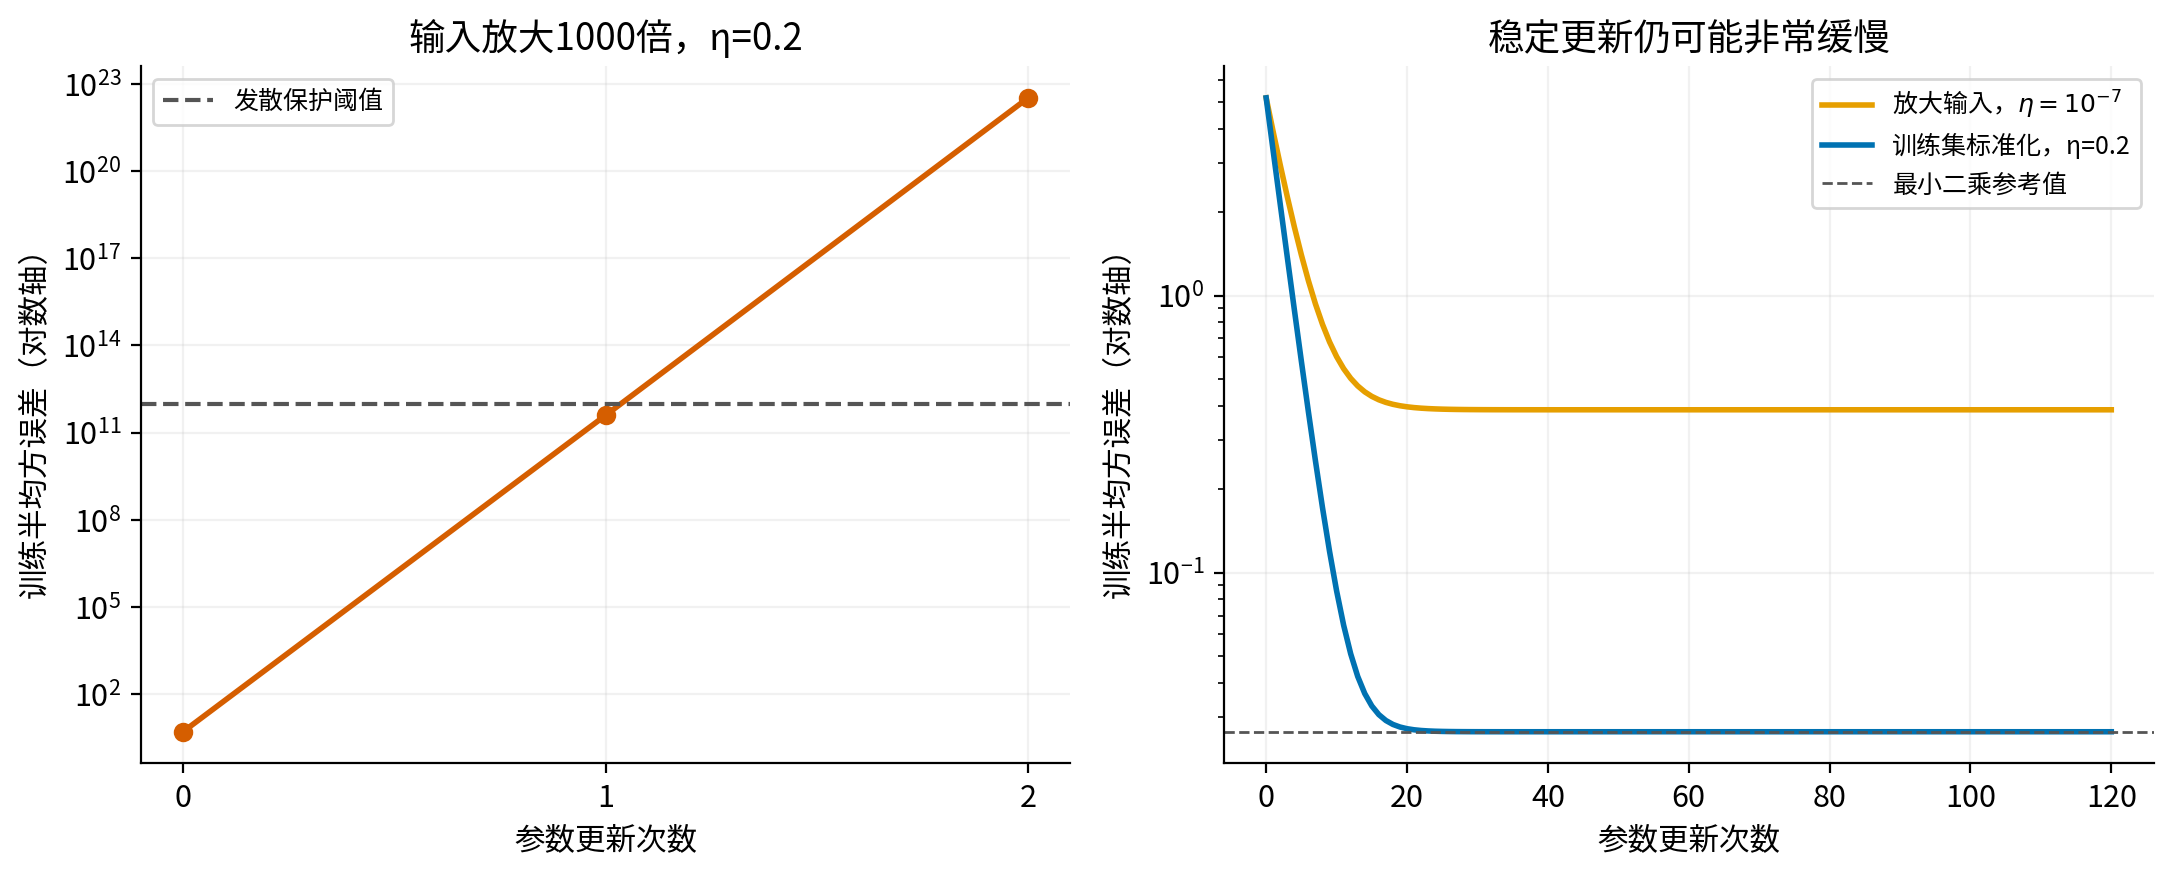
\includegraphics[width=0.92\linewidth]{figures/ch03_figure_4.png}\caption{同一组30条人工训练记录的尺度对照。左图把输入放大1000倍并沿用学习率0.2，在第2步超过发散保护阈值；右图比较放大输入配极小学习率与训练集标准化后的更新。纵轴均为训练半均方误差的对数轴，两幅图范围不同，不能按曲线的视觉高度跨图比较。}\end{figure}

标准化后的系数不能直接与原始坐标的斜率比较。若标准化模型写成 \(\widehat{y} = cz + d\)，其中 \(c\) 和 \(d\) 是新坐标中的斜率与截距，代入 \(z\) 的定义可得：

\[\widehat{y} = \frac{1000c}{s_{u}}x + \left( d - \frac{c\mu_{u}}{s_{u}} \right).\]

因此，原始坐标中的斜率为 \(a = 1000c/s_{u}\)，截距为 \(b = d - c\mu_{u}/s_{u}\)。本次标准化拟合的 \(c \approx 2.989026\)、\(d \approx 1.161905\)，换算后仍得到约2.506900与0.853364。标准化改善了当前优化的数值条件，没有凭空增加数据的信息。这个实验也说明，把不同单位或尺度下的系数数字直接相减，可能会制造没有意义的差异。

\subsection{更换批量方式并解释曲线}

最后，在同一份训练标准化数据上比较三种批量方式。参数都从0开始，学习率都为0.1，均遍历80轮；小批量大小为6，随机打乱种子为42。运行之前，先根据表3-4写出每种方式的更新次数，再预测哪些曲线会更容易出现局部波动。

\begin{figure}[htbp]\centering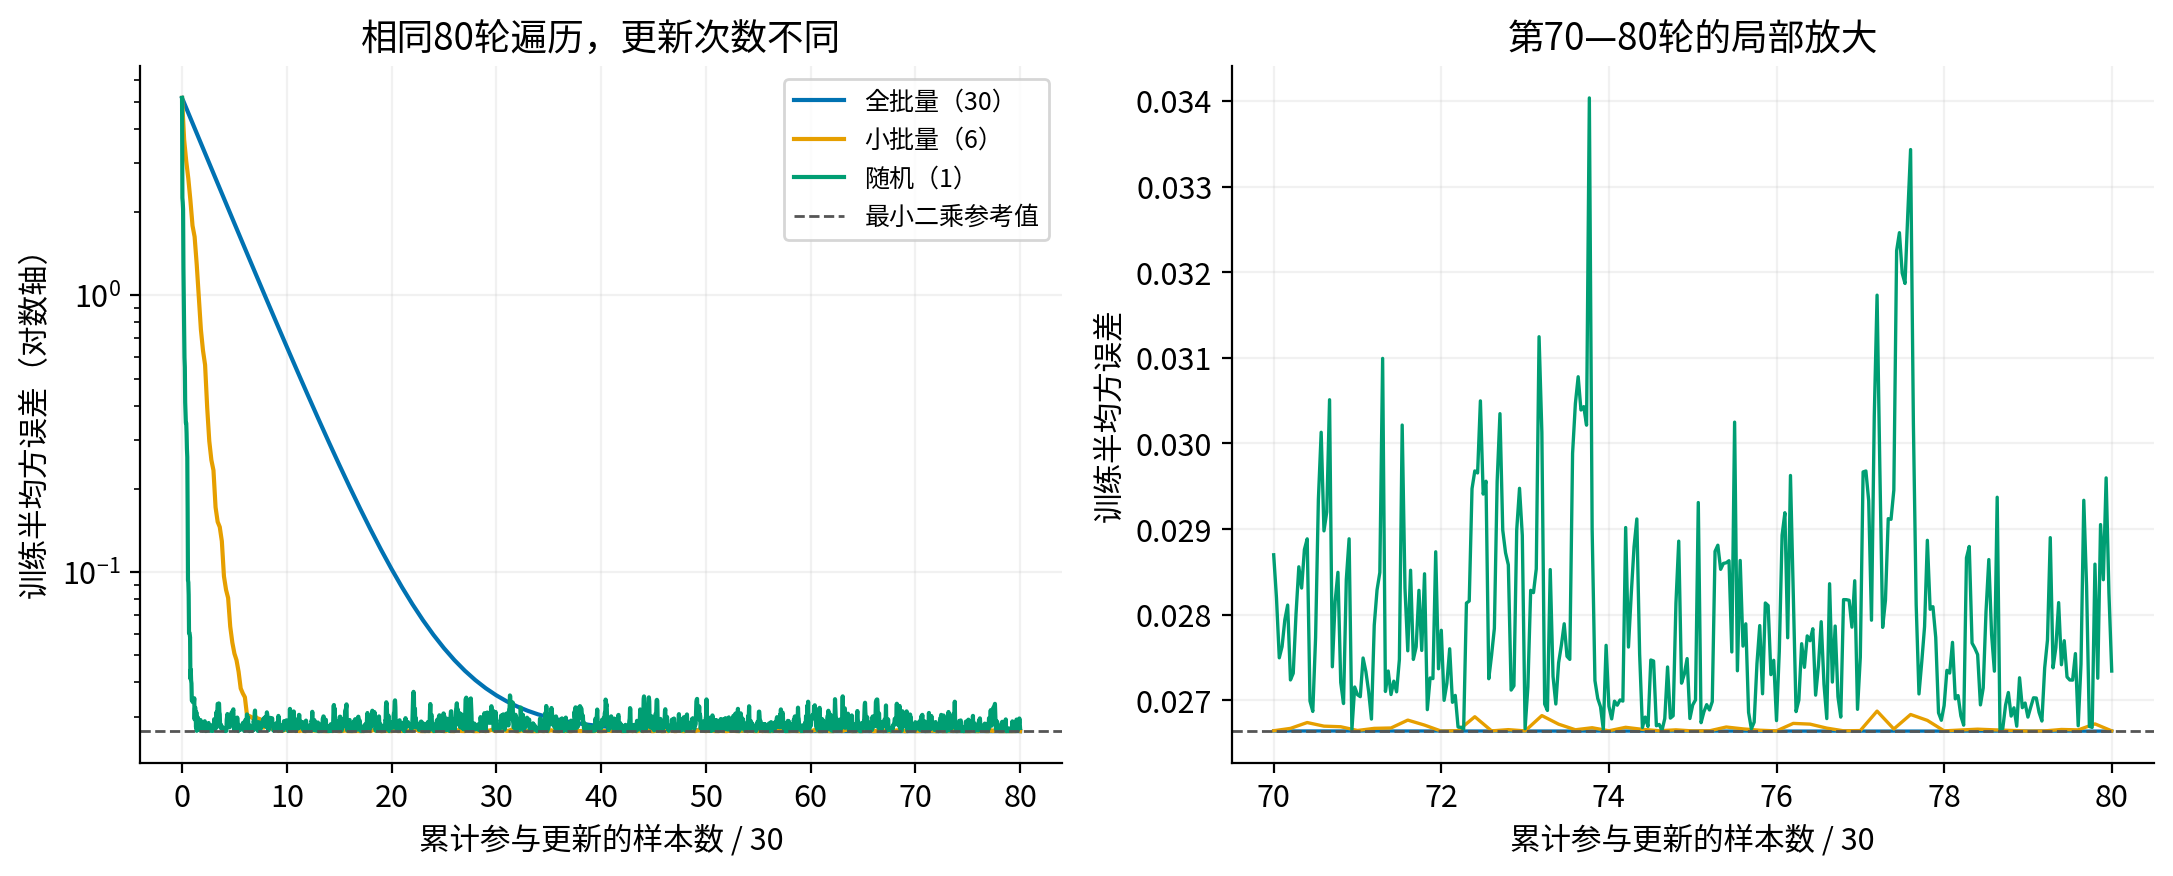
\includegraphics[width=0.92\linewidth]{figures/ch03_figure_5.png}\caption{仅使用30条人工训练记录及由它们拟合的标准化变换。三种方式的常数学习率均为0.1，初值均为0。横轴按累计参与更新的样本数除以30计，整数刻度对应完整遍历轮数；纵坐标始终由全部训练记录计算。右图放大第70至80轮，用于观察最小值附近的波动，不作为运行速度比较。}\end{figure}

图3-5中，单样本更新在相同遍历量内进行了更多次参数调整，早期可以较快靠近较低损失区域；随后仍可看到波动。全批量曲线更平稳，每轮却只走一步。不要用``更平滑''代替``在所有任务中更有效''，也不要用``早期下降快''代替``末步最准确''。它们在这次实验中的差别，是批量大小、学习率和计数方式共同作用的结果。

配套Notebook要求进一步改变打乱种子，观察参数轨迹和末步结果。回答时应明确是哪个目标、哪份数据、哪种计数条件下的现象。例如，可以说``在本次30条训练记录、常数学习率0.1和80轮遍历下，随机更新在最小值附近仍有波动''；不能把一句话缩成``随机梯度下降不收敛''，因为学习率日程、数据特性和训练时长改变后，现象也可能改变。

\subsection{从教学直线走向科学任务}

本实验保留了科学拟合中的几个共同问题：定义输入与目标、选择关系形式、规定误差代价、估计参数并检查残差。若把它迁移到传感器标定，需要进一步讨论量程、系统偏差、重复测量以及不同记录的测量不确定性；若迁移到天文中的经验关系，需要明确样本对象、观测条件和适用范围。我们不会把人工数据上的低训练损失称作某条物理定律得到了验证。

本章的学习结果应当是一条可以解释的链条：参数决定预测，预测产生残差，残差进入损失，梯度描述目标的局部变化，学习率和批量方式规定具体更新，停止条件决定计算何时结束。只会运行最后一行 \texttt{fit} 还不足以说明理解了这条链条；能够借助参数记录解释一条下降或发散的曲线，才为后续模型学习打下了基础。

\subsection{本章练习}

1. 对 \(\widehat{y} = ax + b\)，分别指出输入、监督目标、预测、模型参数和至少三个超参数。如果将学习率从0.2改为0.02，是改变模型表达还是改变优化过程？如果把直线换成二次曲线，又改变了什么？

2. 使用表3-2的三点例子，计算平均残差、MSE与半均方误差，并解释它们的区别。再从 \(a = 1,b = 1\) 出发，用学习率0.3完成一次同步梯度更新，核对新损失。

3. 对示意目标 \(J(w) = (w - 3)^{2}/2\)，从 \(w = 0\) 开始，手算学习率0.5的前两步。再预测学习率2.0的轨迹，运行后说明为什么参数一直变化而损失没有减小。

4. 某程序先更新 \(a\)，然后用新 \(a\) 计算 \(b\) 的梯度。解释它与本章同步更新规则的区别。若这个程序的损失也下降，是否足以证明两者实现相同？

5. 30条训练记录遍历80轮，批量大小分别为30、6和1，各有多少次参数更新？如果另外一个数据集不能被批量大小整除，最后一批的梯度应怎样取平均？

6. 重现尺度实验，解释``大尺度输入与极小学习率''为什么稳定却进展缓慢。把标准化模型的参数换回原始坐标，核对预测是否一致。说明标准化均值和尺度应从哪些记录计算。

7. 保持数据、初值、学习率和轮数不变，把随机打乱种子改为0、1、2、3、4，记录随机与小批量方法的末步训练损失。用结果说明复现一次运行与检查结果波动的区别，不挑选最好的一次代替全部结果。

8. 选择一个熟悉的物理标定或天文经验拟合任务，写出样本单位、输入、目标和拟议模型。列出从本章人工直线迁移过去时，至少三个需要额外检查的问题，并说明为什么训练损失较小不等于科学机制已经成立。

基础提交包括两步参数手算、直线训练记录、学习率和尺度对照图，以及对停止原因的简短解释。批量方式的多种子比较和递减学习率实验可作为进一步探索。教师版Notebook提供参考计算与常见误解的说明。

下一章将暂时放下``怎样继续降低训练损失''，转而建立评价与选择模型的流程。我们会说明怎样使用训练、验证与测试数据，怎样理解过拟合与欠拟合，以及怎样在不接触最终独立测试结果的条件下选择设置。有了这些判断依据，第5章的线性回归、第6章的逻辑回归和第12章的MLP才能放进一套完整而可靠的建模流程中。

\section*{本章参考资料（本章内编号）}

{[}1{]} scikit-learn developers. Stochastic Gradient Descent. 官方用户指南。\url{https://scikit-learn.org/stable/modules/sgd.html} 。关于随机梯度优化、线性估计器及尺度敏感性的说明；本章实际运行版本为scikit-learn 1.8.0，在线stable页面可能随发布更新。

{[}2{]} scikit-learn developers. LinearRegression. scikit-learn 1.8.0 官方API文档。\url{https://scikit-learn.org/1.8/modules/generated/sklearn.linear_model.LinearRegression.html} 。关于最小二乘拟合、构造选项与拟合后系数属性的说明。

{[}3{]} scikit-learn developers. Common pitfalls and recommended practices. scikit-learn 1.8.0 官方用户指南。\url{https://scikit-learn.org/1.8/common_pitfalls.html} 。关于先划分数据、仅在训练部分学习预处理变换及保持变换一致性的说明。

{[}4{]} scikit-learn developers. StandardScaler. scikit-learn 1.8.0 官方API文档。\url{https://scikit-learn.org/1.8/modules/generated/sklearn.preprocessing.StandardScaler.html} 。关于训练均值、尺度及标准差计算约定的说明。

本章数据、表格及数值结果均由配套 \texttt{build\_experiments.py} 实际生成和计算。固定环境、数据字段、运行记录及完整实验位于随章材料；正文取舍以机制解释为主，完整作图与循环代码保留在Notebook中。

\section*{深化练习与方法检验}
本组题强调解释、计算与验证；D编号在本章内独立计数。计算题应写出所用定义和中间步骤，实验题保留实际输出，包括不支持预期的结果。
\begin{enumerate}[label=D\arabic*.]
\item 给定 $J(\theta)=\frac12(4\theta_1^2+\theta_2^2)$，从 $(1,1)$ 出发，以学习率0.2完成一步更新。求常数学习率使任意非最优初值收敛所需的区间，并指出其依据。
\item 将平均平方误差乘以正数5。最优参数、梯度、保持相同更新轨迹所需的学习率分别怎样变化？加入正则化项但不同时缩放其系数时，最优参数是否仍必然不变？
\item 说明“用一个小批量的平均损失估计完整梯度”这句话错在哪里。怎样在合适的随机抽样条件下写出正确的无偏性关系？
\item 某损失曲线几乎水平。提出三种不同解释，并给出能区分它们的进一步检查。
\end{enumerate}
